\documentclass[10pt, b5paper, openany]{ltjsbook}

\usepackage[T1]{fontenc}
\usepackage[utf8]{inputenc}
\usepackage[backend=biber, maxnames=100, backref=true]{biblatex}
\usepackage[binary-units = true]{siunitx}
\usepackage{amsmath, amssymb, amsthm}
\usepackage{graphicx}
\usepackage{hyperref}
\usepackage{ascmac}
\usepackage{here}
\usepackage{comment}
\usepackage{listings}

\setlength{\textwidth}{\fullwidth}
\setlength{\evensidemargin}{\oddsidemargin}

\lstset{
  basicstyle={\ttfamily},
  identifierstyle={\small},
  commentstyle={\smallitshape},
  keywordstyle={\small\bfseries},
  ndkeywordstyle={\small},
  stringstyle={\small\ttfamily},
  frame={tb},
  breaklines=true,
  columns=[l]{fullflexible},
  numbers=left,
  xrightmargin=0\zw,
  xleftmargin=3\zw,
  numberstyle={\scriptsize},
  stepnumber=1,
  numbersep=1\zw,
  lineskip=-0.5ex
}

\DeclareGraphicsRule{.ai}{pdf}{.ai}{}

\title{ \LaTeX Sample1 } 
\author{ komekome09(こめわっぽ) }
\date{ \today }

\begin{document} %document環境
\chapter*{はじめに}
みなさんはゲームをやっていますか?
PCでやるゲームと言えば、アクションゲーム、リズムゲーム、RPGなどがありますが、この本で扱うのはいわゆるノベルゲームと呼ばれるタイプのゲームについてです。

例えばみなさんは以下のような経験をしたことはありませんか?
\begin{itemize}
    \item 自宅のWindows機でやっているゲームを出先でもやりたいがMacしか持ってなくてできない……!
    \item Windowsしか対応してないけど宗教上の理由でWindowsが使えない… Vineだと動かないし…
\end{itemize}
こんなときにOSなどのプラットフォームに依存しないような実行環境があったら良いと思いませんか?
筆者は(学会などで遠出した際に)感じることがありました。

プラットフォーム非依存の環境で動作させるとなるとQtやJavaなどのクロスプラットフォームを採用しているソフトやライブラリで開発をすれば可能です。
しかし今までに発売されたソフトの中にはWindowsでしか動かないようなソフトも当然ありますし、それらのソフトに対する答えにはなりえません。

そこでこの本ではOSに依存しない環境で(主にWindows専用ソフトを対象とした)ノベルゲームを実行するためのプラットフォームを作ろうと奮闘した本です。
内容的にはまだまだですが、筆者が本を作ってみたいなどの個人的な都合などもあり、筆を取ることにしました。
本の内容としてはUEFIの基本的な内容から実際にどのように実装したのかまでを(なるべく)詳しく書いてみました。
誤字や誤記、間違いなどもあるかもしれませんが、見つけた時は遠慮なく教えていただけると幸いです。

\tableofcontents
\clearpage

\chapter{デモ}
\begin{figure}[H]
    \centering
    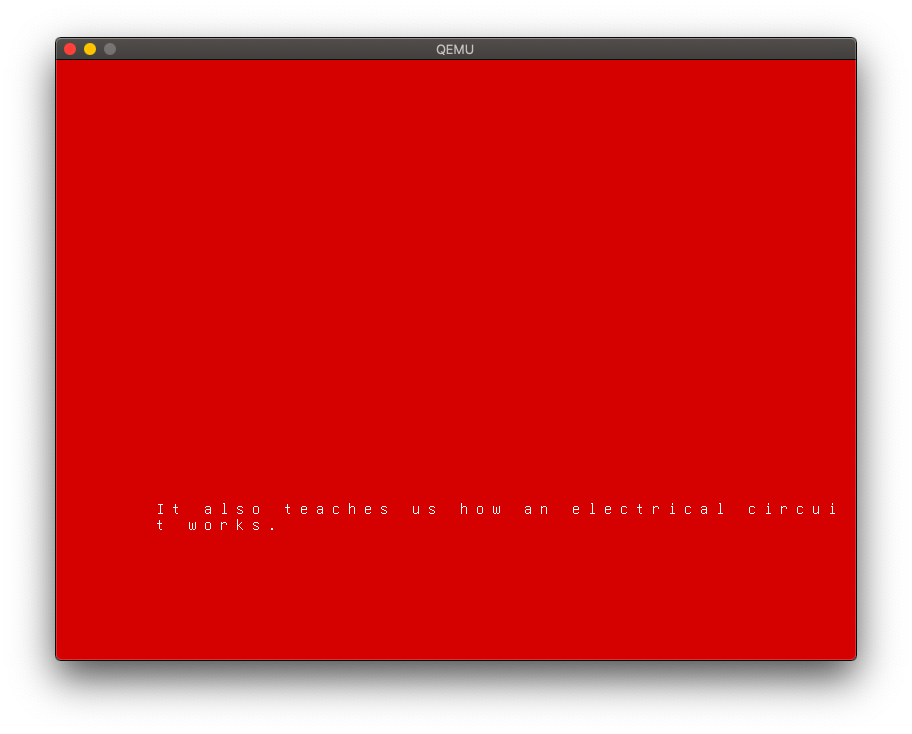
\includegraphics[scale=0.3]{pic/screenshot.png}
    \caption{作成中の画面}
    \label{fig:screenshot}
\end{figure}
本の執筆時点では画像、テキストなどのファイルの読み込み、画像の表示、フォントの表示、キー入力はできています。
反対に音声ファイルや画像の透過などには未対応です\footnote{デモ機の時点では少しは進んでいるかもしれません}。

\chapter{そもそもUEFIとは?}
UEFIはUnified Extensible Firmware Interfaceの略で、OSとプラットフォームファームウェア間を結ぶインターフェースのことを指します。
一言で言うとBIOSの後継のようなものですが、BIOSの機能とは全く異なるものとなっています。
BIOSでは基本的にOSのロードを行うブートローダーとしての役割がほとんどでしたが、UEFIではそのロードの前段階であらかじめ用意された多くの機能を扱うことができます。
また様々なハードウェア上で動作するように設計されているため、移植が比較的容易であるという利点もあります。

元々はIntelが1998年に開始したIntel Boot Initiativeが元になっており、2000年にEFIの仕様書が始めて作成されました
\footnote{ただしこれは法的に問題があったため、2002年のバージョンアップからが正式となっています}。
現在の最新バージョンは2.8です。

この本では、提供されるランタイム機能を駆使してUEFIアプリ(ノベルゲーム)を作成します。
そのUEFIアプリを作るのは別に仕様書を片手に全部1から書くことができますが、普通は開発用のツールが提供されています。
UEFIアプリでは主にEDK2とgnu-efiの2つが有名なツールです。

EDK2は多機能でlibcやmrubyなどが使えます。
ただビルドの方法が分かりにくく、とっつきやすさはgnu-efiの方が上に思えます。
gnu-efiは機能としてはEFIのインターフェースのみをまとめており最低限の機能しかありませんが、その分かりやすいです。
ただ自分で実装する量は増えます。
この本ではgnu-efiを用いて開発を行うことにしました。

\chapter{(最終的な)実装内容}
UEFIアプリ上でノベルゲームの土台を作るという目標ですが、具体的にどのような機能を実装すればいいのかを以下に示しました。
\begin{itemize}
    \item ファイル処理(読み書き)
    \item 画像処理(表示)
    \item BGM
    \item テキスト(フォント等)
    \item キー入力
\end{itemize}
まずはこれを足掛りとして考えていきます。

\section{ファイル処理}
ファイル処理はEFIインターフェースで提供されています。
そのため、仕様書に従って実装するだけで機能を実現できます。

\section{画像処理}
画像処理は表示するだけならEFIインターフェースで可能です。
表示には各ピクセルのRGBデータを得る必要がありますが、画像ファイルが圧縮されている場合などは解凍処理などを実装する必要があります。
また、透過処理(アルファブレンドなど)も実装が必要となります。
ノベルゲームなどでは図\ref{fig:nobel_exp}に示すようにテキストを表示する枠の部分(ピンク色)が背景画像(橙色)に対して透過していることが多々あるため、機能としては必須と考えています。
\begin{figure}[H]
    \centering
    \includegraphics[scale=0.3]{pic/nobel_exp.ai}
    \caption{ノベルゲームの表示例}
    \label{fig:nobel_exp}
\end{figure}

\section{BGM}
BGMに関してはUEFIが提供しているインターフェースに音楽などの再生機能が無いため、ドライバ経由でアクセスするなどの手段を自力で実装する必要があります。
実装方法としてはPCスピーカーを使う方法がもっとも単純ですが、いわゆるビープ音しか鳴らせないためHDA(High Difinition Audio)インターフェースに対応することでより高音質なデータを扱うことができます。

\section{テキスト}
インターフェース自体にも文字の出力関数は容易されていますが、画像で塗り潰してしまうため見えなくなるというのと、見栄えが非常に悪くなるという問題があります。
\begin{figure}[H]
    \centering
    \includegraphics[scale=0.3]{pic/nobel_exp.ai}
    \caption{標準インターフェースでの文字の表示例}
    \label{fig:text}
\end{figure}
そのため、フォントを画像として表示することで各種問題を回避しています。
今回はGNU Unifontのビットマップ画像を用いたフォント表示を実装することにしました。
ビットマップフォントなので見た目はよろしくありませんが、背景色で透過できるためより自然な見た目になります(デモの章の画像のような感じになります)。
将来的にはTrueTypeフォントを扱えるようにできればより綺麗にフォントを表示できるようになります。

\chapter{環境構築}
では実際にUEFI Applicationを作るための開発環境を構築していきます。

筆者の環境を下記に示します。
\begin{table}[H]
    \centering
    \begin{tabular}{|c|c|}
        \hline
        PC & MacBook Air (13-inch, Early 2015) \\
        CPU & Intel Core i5-5250U @ 1.60GHz \\
        Memory & 8GB DDR3 \\
        OS & macOS Mojave 10.14.5 \\
        \hline
    \end{tabular}
\end{table}
使用するソフトは、
\begin{itemize}
    \item gcc 8.2.0
    \item curl 7.63.0 (x86\_64)
    \item Docker Desktop Community Ver. 2.0.0.3 (31259)
    \item QEMU emulator version 4.0.0
\end{itemize}
です。
ライブラリは gnu-efi 3.0.9 を使用します。

実行ファイルはPE32+形式ですが、クロスコンパイラ等は使用せずにコンパイルを行います。
そのため今回はDocker上に開発環境を作成しました。
DockerFileなどを含めたソースコード類はGitHubに上げています\footnote{\url{https://github.com/komekome09/efi-story}}。
見てもらえれば分かりますが、まあなんの変哲もない普通のDockerfileです。

このコンテナではコンパイル部分のみを実行し、実際のコード編集と実行はホスト上で行うようにしています。
そのためコンテナとホストでdocker-composeを使って開発ディレクトリを共有しています。
この方式を取った理由は簡単で、ホスト側の環境がめちゃくちゃにならなくて済むからです。
将来的にはclangから直接PE32+形式のファイルを生成する形に変更するつもりです。
そうすればDockerも必要なくなります\footnote{詳しくは\url{https://dvdhrm.github.io/2019/01/31/goodbye-gnuefi/}参照}。

コード編集から実行までの流れは、
\begin{enumerate}
    \item コードを編集する
    \item dockerコンテナを実行してコンパイル $\rightarrow$ 共有ディレクトリにファイルが生成される
    \item ホスト上で実行(今回はqemu)
\end{enumerate}
となります。

\chapter{コード}
\section{画像処理}
UEFI上での描画には、\verb+EFI_GRAPHICS_OUTPUT_PROTOCOL+というプロトコルを利用します。
より具体的には、ピクセルデータである\verb+EFI_GRAPHICS_OUTPUT_BLT_PIXEL+構造体に色データを代入し、それをフレームバッファーに描きこむことで描画します。
フレームバッファーにはアドレスを取得して直接書き込む方法もありますが、今回はダブルバッファリング(描画メモリと別のメモリ上との)を行う方法を使っています。

画像ファイルはファイルが置いてある場所(ボリューム)から読み込み、RGBの画像データに変換する必要があります。
現在の主流フォーマットはおおむね圧縮されていたりするのでこれを解凍する処理も必要となります。
これを全部書くのはとてもではないですが現実的では無く、終わる気配が無くなってしまうので(興味はあるのですが…)今回はnothings氏が作成したstbと呼ばれる単一ファイルから構成されるライブラリを利用しました\footnote{\url{https://github.com/nothings/stb}}。
このライブラリもlibcを利用しているため、libc関連の処理は全て置き換える必要があります。
正確な数は数えていないので分かりませんが、この程度の行数であればそこまで多くは無いでしょう(最低限の所のみ置き換えしている)。

本来であればlibcのラッパーを書く or EDK2を使うのが一番手っ取り早いと思います(EDK2にはlibcのラッパーがあります)。
EDK2を使わなかった理由はどうせ作るなら自分で色々書きてえよなあという単純な考えです(最近はgnu-efiすらやめようと考えてすらいます)。

という話は置いておいて、実際の処理の話をしていきます。

処理の流れとしては以下のようになります。
\begin{itemize}
    \item ファイルのあるボリューム(ディレクトリ)を開く
    \item メモリにファイルを読み込む
    \item ライブラリを利用して別のメモリ領域に画像データとして読み込む
    \item フレームバッファに書き込み
    \item ディスプレイに描画
\end{itemize}
この処理を繰り返すことで描画を行います。

ボリュームはOpenVolume関数で開きます。

\section{フォント処理}

\section{キー処理}

\chapter{あとがき}

\begin{comment}
\section{見出し1}
    本文はこんな感じで入力します。\par
    改行をしたいときは、字下げを行う場合は \verb+\par+ 、そうでない場合は\verb+\\+ を使います。
    \subsection{小見出し1}
        見出しの中をさらに小分けができます。こういった分け方を「章立て」と呼び、日本語では大きい単位から「章」「節」「項」と言います。\par
        \LaTeX ではデフォルトでは1.1.2、といった形で表示され、この場合は第1章第1節第1項、と呼びます。
        \subsubsection{小々見出し1}
        \LaTeX{} is a document preparation system for the \TeX{} typesetting program. It offers programmable desktop publishing features and extensive facilities for automating most aspects of typesetting and desktop publishing, including numbering and cross-referencing, tables and figures, page layout, bibliographies, and much more. \LaTeX{} was originally written in 1984 by Leslie Lamport and has become the dominant method for using \TeX; few people write in plain \TeX{} anymore. The current version is \LaTeXe.
\section{基本的な文法}
    \subsection{箇条書き}
        箇条書きにはいくつか種類があります。
        \subsubsection{itemize}
            これは「・」が頭についた箇条書きです。
            \begin{itemize}
                \item 箇条書き1
                \item 箇条書き2
                \item 箇条書き3
            \end{itemize}
        \subsubsection{enumerate}
            これは頭に数字が振られている箇条書きのコマンドです。
            \begin{enumerate}
                \item 箇条書き1
                \item 箇条書き2
                \item 箇条書き3
            \end{enumerate}
        \subsubsection{description}
            これは頭につける記号をユーザが決めることができるコマンドです。
            \begin{description}
                \item[テスト1] 箇条書き1
                \item[テスト2] 箇条書き2
                \item[テスト3] 箇条書き3
            \end{description}
    \subsection{表組み}
        \subsubsection{基本的な表}
            \begin{table}[H]
                \begin{center}
                \caption{基本的な表}
                \begin{tabular}{|l|c|r|}
                    \hline
                    セル1 & セル2 & セル3 \\ \hline
                    セル4 & セル5 & セル6 \\ \hline
                    セル7 & セル8 & セル9 \\ \hline
                \end{tabular} 
                \end{center}
            \end{table}
        \subsubsection{セルの結合}
            \begin{table}[H]
                \begin{center}
                \caption{セルの結合}
                \label{tab:sample1}
                \begin{tabular}{|l|c|r|}
                    \hline
                     & \multicolumn{2}{|c|}{セル1} \\ \cline{2-3}
                    セル2 & セル3 & セル4  \\ \cline{2-2}
                     & セル5 &  \\ \hline
                \end{tabular} 
                \end{center}
            \end{table}
            表を参照するときはこうします(表\ref{tab:sample1})
        \subsubsection{複数の表}
        \begin{table}[H]
            \begin{center}
            \begin{tabular}{cc}
            
            \begin{minipage}{0.5\hsize}
            \begin{center}
            \begin{tabular}{|c|c|c|}
            \hline
            a & b & c \\ \hline
            d & e & f \\ \hline
            g & h & i \\ \hline
            \end{tabular}
            \caption{aが9つ}
            \end{center}
            \end{minipage}
            
            \begin{minipage}{0.5\hsize}
            \begin{center}
            \begin{tabular}{|c|c|c|}
            \hline
            j & k & l \\ \hline
            m & n & o \\ \hline
            p & q & r \\ \hline
            \end{tabular}
            \caption{bが9つ}
            \end{center}
            \end{minipage}
            
            \end{tabular}
            \end{center}
        \end{table}
    \subsection{数式}
        \subsubsection{その1}
            \begin{eqnarray}
                G_{-1}(x,y)=x^{n-1}+x^n-1
                \label{eq:sample1}
            \end{eqnarray}
                
            \begin{eqnarray}
                W(D)&=&(I(D),(1+D)I(D)) \nonumber \\
                &=&I(D)[1,1+D] \nonumber \\
                &=&I(D)G(D)
            \end{eqnarray} 
            
            \[
            x=a+b+c
            \]
            
            本文中にも数式を$ x=a+b+c $表示できます。\par
            数式の参照はこうやります(式(\ref{eq:sample1}))            
        \subsubsection{その2}
            \begin{eqnarray}
                y=\frac{\sqrt[2]{1+x}}{1-x}
                \end{eqnarray} 
                
                \begin{eqnarray}
                \left(\frac{1+x}{1-x}\right) +(\frac{1-x}{1+x})
                \end{eqnarray} 
                
                \begin{eqnarray}
                c_{k,l}=\left\{ \begin{array}{ll}
                1[\mathrm{m/s]}] & (l=k) \\
                \alpha & (|l-k|=1) \\
                0[\mathrm{m/s]} & (上記以外) \\
                \end{array} \right.
            \end{eqnarray}
    \subsection{画像の挿入}
        \begin{figure}[H]
            \begin{center}
            %\includegraphics[width=5cm]{figure1.jpg}
            \end{center}
            \caption{図の説明}
            \label{fig:sample1}
        \end{figure}
        画像の参照はこうやります(図\ref{fig:sample1})
\section{参考文献の参照}
    参考文献を参照する場合は\cite{bib1}こうします。
\section{その他のコマンド}
    その他特殊文字や細かい操作方法などは\cite{sheat1,sheat2}を参照してください。

\begin{thebibliography}{9}
    \bibitem{bib1} ここに参考文献を入力します
    \bibitem{sheat1} unknown, `` LaTeXコマンドシート一覧,'' 2003, [online] Available: \url{http://www002.upp.so-net.ne.jp/latex/index.html}
    \bibitem{sheat2} unknown, `` LaTeXコマンド集,'' 2009, [online] Available: \url{http://www.latex-cmd.com}
\end{thebibliography}
\end{comment}
\end{document}

